\section{Homework}

\textbf{Exercise 1 - Finding Dependencies} \\
Find the dependencies in the code in appendix A that could make testing hard. Give reason. 

\begin{itemize}
    \item The properties for the database connection are directly hardcoded in the source code. With this, it would not be possible to inject a mock database.
    \item The webservice call (TierUtil) is directly implemented in the same method, which makes it hard to fake it.
    \item The statement for the query is built and executed in the same method as the rest. This makes it hard to test the statement or mock the execution of the statement.
\end{itemize}

\textbf{Exercise 2 - Finding Seams} \\
Find the seams and enabling points in the code in appendix A. \\
\textit{a seam is a place where you can change the behavior without editing in that place
every seam has an enabling point, a place where you can make the decision to use one behavior or another}

\begin{itemize}
    \item The database connection could be used as seam point. Its enabling point is the constructor, which takes a connection argument as parameter.
\end{itemize}

\textbf{Exercise 3 - Get Class under Test} \\
How can we get class Customer in Appendix A into Test Harness? Discuss possible solutions with your neighbor. 

Generally, one needs to break the dependencies in that class to be able to test the parts of it seperately. 

\begin{itemize}
    \item Extract and Override Call: Extract the call to a virtual method and then override it in a testing subclass
    \item Extract and Override Factory Method: Extract object creation into factory method and override in tests
    \item Replace Global Reference with Getter: Extract global reference to method and override in tests
    \item Extract Interface: Find member functions to extract, and copy function signatures to a interface
    \item Parameterize method: Identify dependency and make new method with arguments
\end{itemize}

\textbf{Exercise 4 - Get Method to run under Test} \\
Execute all necessary measures to break dependencies to be able to run the method ratePolicy(..) under test in isolation.

Directly commented in the code.

\columnbreak

\begin{lstlisting}[language=Java]
class Customer{
    private TierUtil tierUtil;
    private RGHConnection connection;
    public Customer(RGHConnection con)
    {
        //EXEC 4: this.connection = con;
    }
    /* EXEC4 ADDITIONALS

    private void createTierUtil(){
        this.tierUtil = new TierUtil();
    }
    
    private void publishContentOnWebService(int birthyear, int score){
        this.tierUtil.assignTier(birthyear, score);
    }
    
    private Statement createDbQuery(){
        ...
    }
    
    private ResultSet executeDbQuery(Statement stmt){
        ...
    }
    END OF ADDITIONALS */
    
    public Policy ratePolicy(Policy policy, Customer customer) {
        Rater rater = null;
        if (policy.getState().equals("NY")) {
            rater = new NYRater();
        } else if (policy.getState().equals("CA")) {
            rater = new CARater();
        }
        TierUtil tierUtil = new TierUtil(); // Note: This makes a Web Services
        // EXEC4: Leave following initialization of DB away.
        String url = "jdbc:mysql://localhost:3306/";
        String dbName = "policydb";
        String driver = "com.mysql.jdbc.Driver";
        String userName = "policyapp";
        String password = "prodpass";
        try {
            Class.forName(driver).newInstance();
            connection = DriverManager.getConnection(url+dbName, userName,password);
            connection.close();
        } catch (Exception e) {
            e.printStackTrace();
            return null;
        }
        //EXEC4: Outsource following code block into new methods above
        Statement stmt = connection.createStatement();
        ResultSet srs = stmt.executeQuery(
        "SELECT NAME2, NAME1, BIRTHYEAR, SCORE, STATE
        FROM POLICIES WHERE CUST=" + policy.getId());
        policy.setLastName(srs.getString("NAME2"));
        policy.setFirstName(srs.getString("NAME1"));
        policy.setRate(rater.rate(srs.getString("STATE"),
        tierUtil.assignTier(srs.getString("BIRTHYEAR"), srs.getString("SCORE"))));
        return policy;
    }
}
public class RGHConnection
{
    public RGHConnection(int port, String name, string passwd)
    IOExecption{...}
    ...
}
\end{lstlisting}

\clearpage

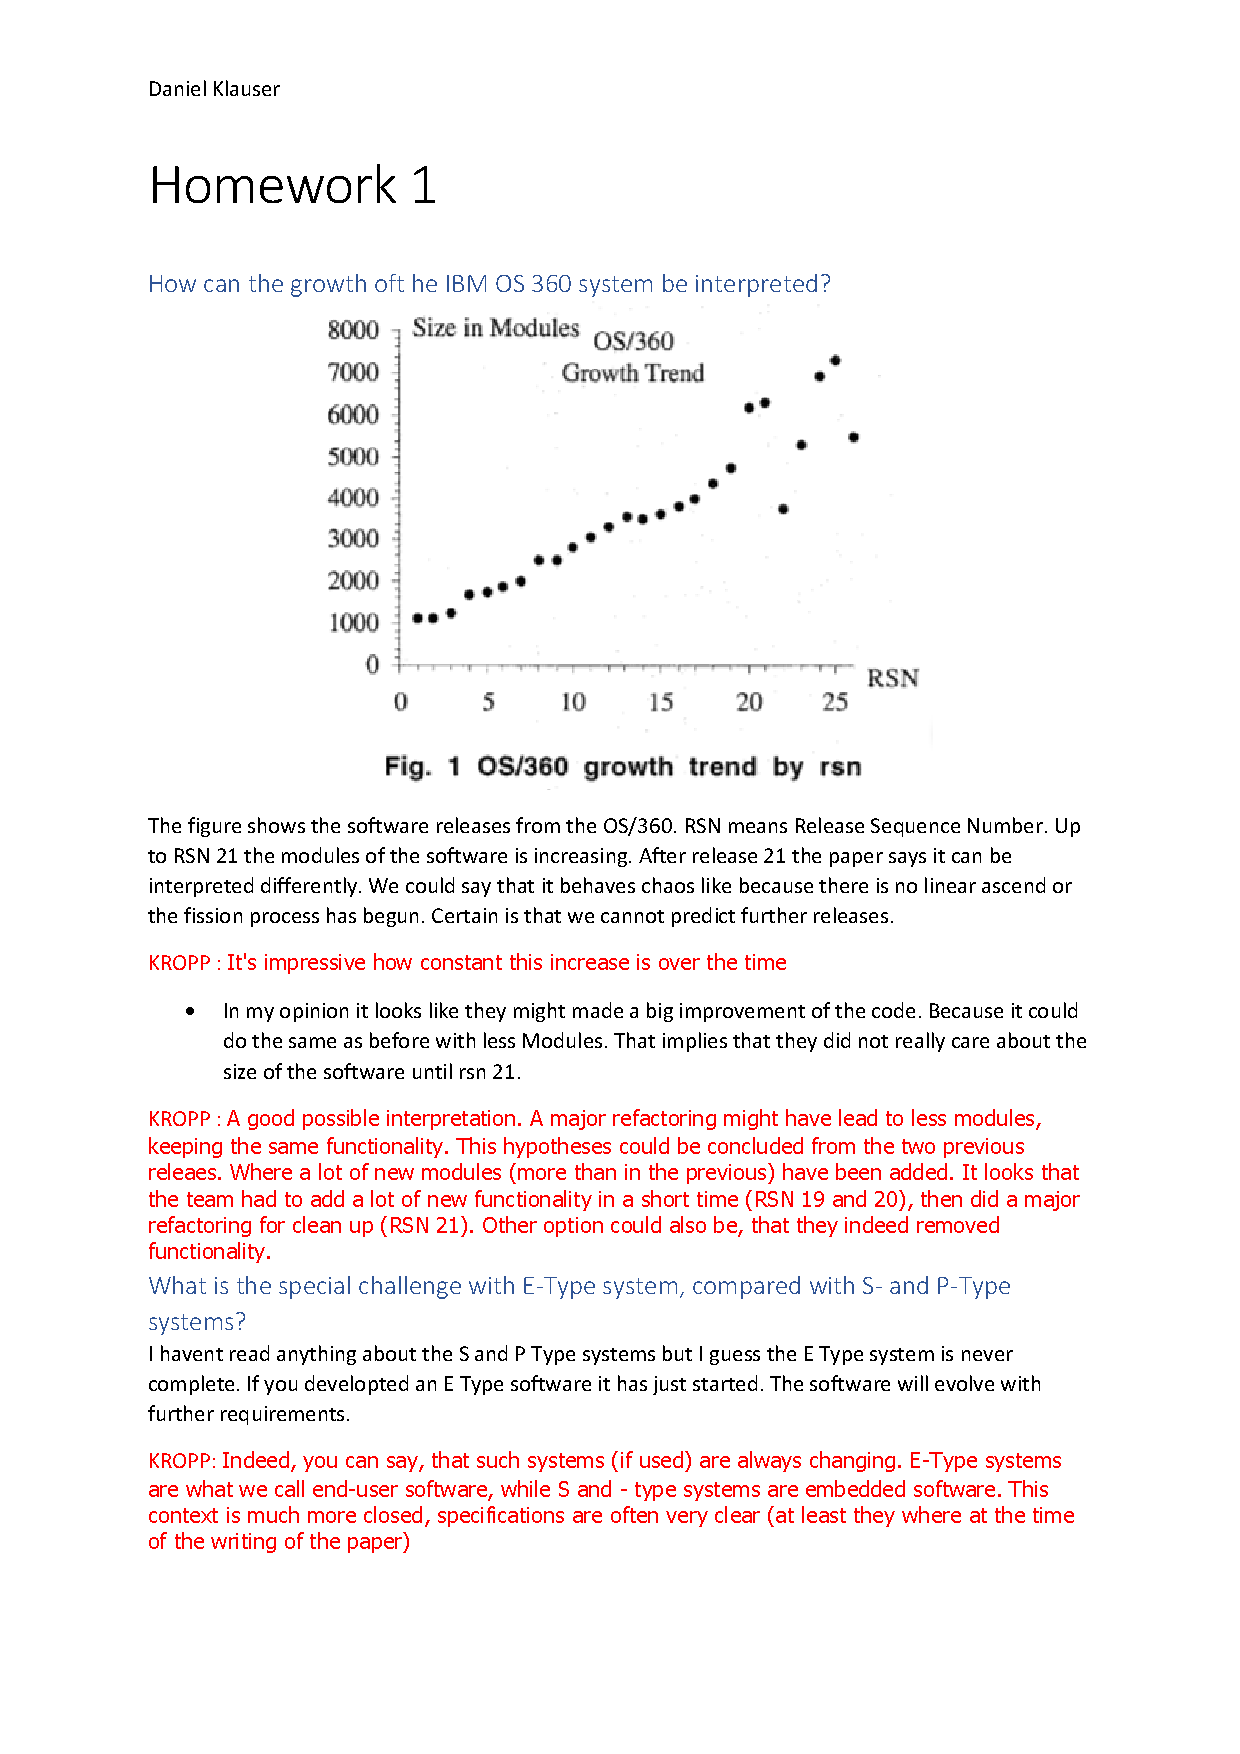
\includepdf[pages=-]{figures/SoftwareEvolution_Task1Kropp.pdf}
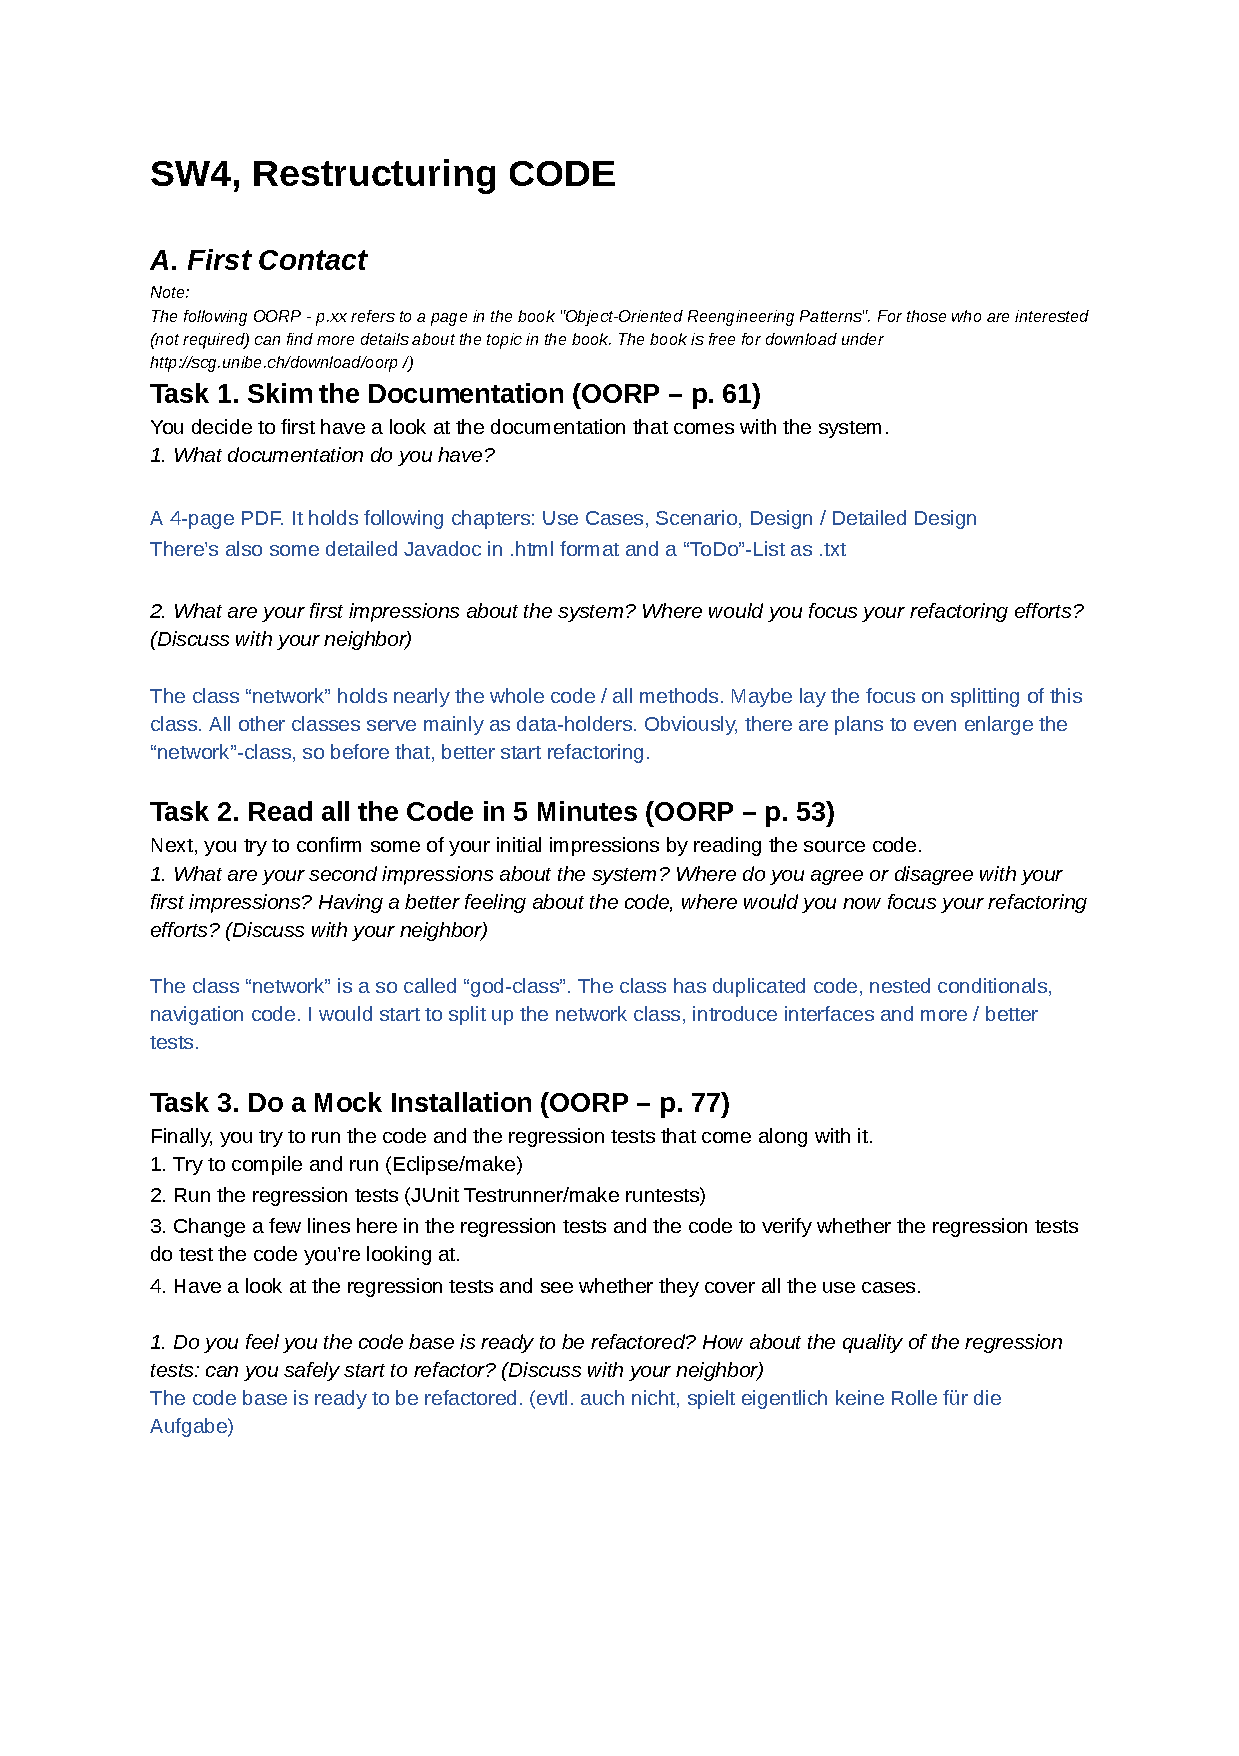
\includepdf[pages=-]{restOfExercises.pdf}